\documentclass[12bp]{guo}
\usepackage{guo}
\usepackage{minted}
\usepackage{titlesec}
\usepackage{indentfirst}
\usepackage[epsilon]{backnaur}
\usepackage[labelformat=empty]{caption}

% source code listing
\usemintedstyle{vs}

% title
\titleformat
{\section}
[block]
{\fontlf}
{}
{0ex}
{}
[]
\setcounter{section}{0}

\titleformat
{\subsection}
[block]
{\fontli}
{}
{0ex}
{}
[]
\setcounter{subsection}{0}

\titleformat
{\subsubsection}
[block]
{\fontlj}
{}
{0ex}
{}
[]
\setcounter{subsubsection}{0}

% figure
\renewcommand{\figurename}{}
\renewcommand{\thefigure}{}

\begin{document}

\section{实验一 进程调度}

\subsection{1、 实验目的}

使用高级语言编写和调试一个进程调度程序,以加深对进程的概念及进程调度算法的理解。

\subsection{2、 实验内容及要求}

进程调度算法:采用最高优先数优先的调度算法(即把处理机分配给优先数最高的进程)
和多级响应队列调度算法。


每个进程有一个进程控制块( PCB)表示。进程控制块可以包含如下信息:
进程名、优先数、到达时间、需要运行时间、已用CPU时间、进程状态等等。


进程的优先数及需要的运行时间可以事先人为地指定(也可以由随机数产生)。
进程的到达时间为进程输入的时间。


进程的运行时间以时间片为单位进行计算。


每个进程的状态可以是就绪 W(Wait)、运行R(Run)、或完成F(Finish)三种状态之一。


就绪进程获得 CPU后都只能运行一个时间片。用已占用CPU时间加1来表示。


如果运行一个时间片后,进程的已占用 CPU时间已达到所需要的运行时间,则撤消该进程,
如果运行一个时间片后进程的已占用CPU时间还未达所需要的运行时间,
也就是进程还需要继续运行,此时应将进程的优先数减1(即降低一级),
然后把它插入就绪队列等待CPU。


每进行一次调度程序都打印一次运行进程、就绪队列、以及各个进程的 PCB,以便进行检查。   


重复以上过程,直到所要进程都完成为止。

\subsection{3、 实验设计方案及原理}

因为本实验需要进行进程调度模拟,所以需要程序需要分拆两个主要模块:

\begin{enumerate}
    \item[(1)] 进程生成:可以根据不同生成算法来模拟进程生成、销毁的过程。
    \item[(2)] 进程调度:使用不同的调度算法来对所有进程进行调度。
\end{enumerate}


\subsubsection{进程生成}

对于每一个进程,可以划分为两个维度:

\begin{enumerate}
    \item[a.] 所需时间片大小
    \item[b.] 运行优先度大小
\end{enumerate}


为了模拟这些数值,程序提供了均值分配、递增分配和正态分布分配三种生成算法,
运行时可以按照需要指定所使用的算法。


\subsubsection{进程调度}

程序实现了 round robin 调度、最高优先度优先和多级反馈队列三种调度算法。
尽管三种算法调度方案不同,但总体运行流程框架均可以概括为:

\begin{enumerate}
    \item[(1)] 从待运行进程队列中选取一个进程
    \item[(2)] 执行该进程
    \item[(3)] 根据进程状态将其放入待运行队列或已完成队列
    \item[(4)] 重复 (1) 直到待运行进程队列为空
\end{enumerate}


\subsection{4、 程序流程图}

\subsubsection{round robin 调度}

\begin{figure}[h!]
    \centering
        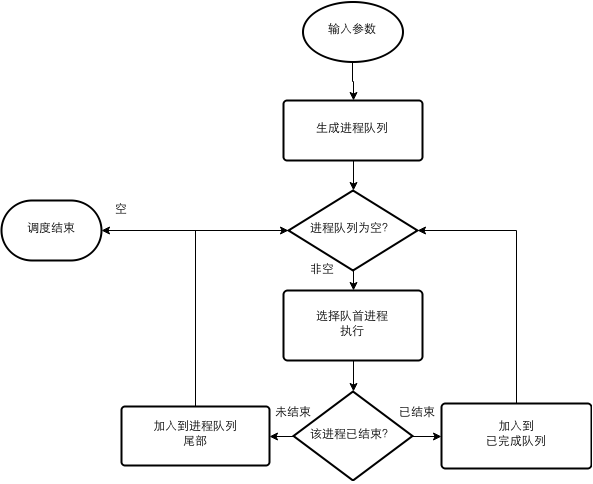
\includegraphics[scale=0.75]{figures/1.flow.rr.png}
\end{figure}

\subsubsection{最高优先度调度}

\begin{figure}[h!]
    \centering
        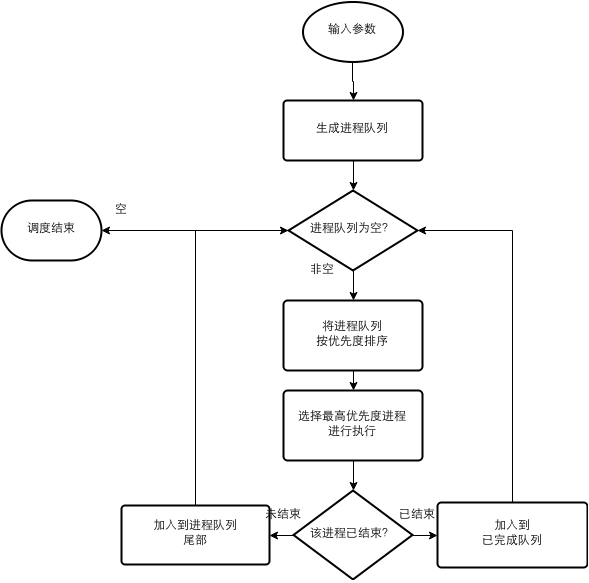
\includegraphics[scale=0.75]{figures/1.flow.priority.png}
\end{figure}


\subsection{5、 程序调用关系}

对于三个调度算法测试程序,在接收用户输入之后都会调用
\mintinline{c}{PREPARE_PROCS} 函数来生成测试进程。


之后程序会转入到 \mintinline{c}{schedule} 函数开始进行调度。
不同算法实现可以根据需要调用进程相关处理函数(例如 \mintinline{c}{proc_info})
来对进程进行控制;并使用 \mintinline{c}{proc_run} 函数来执行一个进程。


调度结束之后,程序需要执行 \mintinline{c}{proc_destory_list} 函数来销毁进程列表。


\subsection{6、 数据结构及疑难描述}

\subsubsection{进程控制块}

进程控制块记录的是进程基本信息,其中包括以下几个字段:

\begin{table}[H]
    \centering
    \begin{tabular}{| c | c | l |}
        \hline
        字段名 & 类型 & 作用 \\ \hline
        pid & int & 进程标志符 \\
        state & int & 进程状态(等待中、运行中、运行完毕) \\
        name & char * & 进程名称 \\
        priority & double & 进程优先度 \\
        ntime & int & 进程所需时间片\\
        rtime & int & 进程已经运行的时间片 \\ \hline
    \end{tabular}
\end{table}

这样各个调度算法可以根据自身需要对进程列表进行排序、选择执行进程。

\subsubsection{正态分布生成算法}

为了更好地模拟真实场景的进程调度情况,可以采用正态分布曲线来模拟进程的优先度
和时间片长度。


实验中使用了 Marsaglia polar method 来模拟正态分布曲线的生成。

\subsubsection{进程队列排序算法}

因为进程队列使用了指针的数据结构,为了更加方便实现进程队列的反复排序,
实验中采用了归并排序。


归并排序的优点在于对链表结构排序方便,时间复杂度为 $ O(n log n) $


\subsection{7、 程序运行结果}

实验中,每个调度算法都有对应的可执行程序,并可以通过命令行参数指定进程数、
优先度生成算法和时间片长度生成算法。


以 round robin 算法为例,可以通过以下命令来指定程序创建 2 个进程,
并使用均值分配时间片、正态分布分配优先度:

\begin{minted}{shell}
    $ ./round_robin_sched 2 MEAN NORM
\end{minted}

以下均以上述参数组合来执行各个调度算法:

\subsubsection{round robin 调度算法}

\begin{figure}[h!]
    \centering
        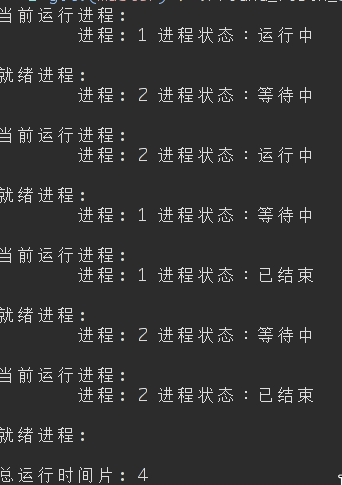
\includegraphics[scale=0.75]{figures/1.rr.png}
\end{figure}

\clearpage

\subsubsection{最高优先度优先调度算法}

\begin{figure}[h!]
    \centering
        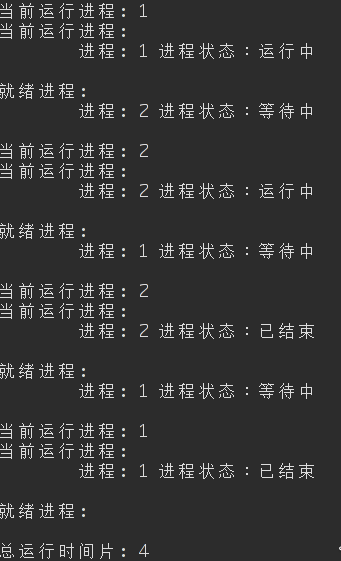
\includegraphics[scale=0.75]{figures/1.priority.png}
\end{figure}

\clearpage

\subsubsection{多级响应队列调度算法}

\begin{figure}[h!]
    \centering
        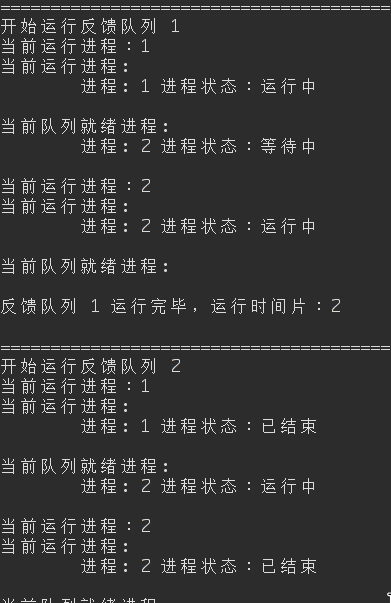
\includegraphics[scale=0.75]{figures/1.multi.png}
\end{figure}


\subsection{8、 结果分析与实验小结}

通过实验中的多次测量检查,可以看到三个不同调度算法都按照预期效果执行。
但对于不同规模的数据不同调度算法有不同表现;例如最高优先度优先算法在执行过程中
响应度较高,而 round robin 调度算法则实现直观简单,性能也尚算可以。多级反馈队列
则兼顾了最高优先度优先、 round robin 算法两者的优点,但实现起来比较复杂,
需要使用更多的数据结构支持。


通过本次实验,加深了我对进程调度算法的理解和体会,并通过学习不同调度算法的实现,
提高了我的编码能力。



\clearpage

\section{实验二 作业调度}

\subsection{1、 实验目的}

用高级语言编写和调试一个或多个作业调度的模拟程序,以加深对作业调度算法的理解。

\subsection{2、 实验内容及要求}

由于在单道批处理系统中,作业一投入运行,它就占有计算机的一切资源直到作业完成为止,
因此调度作业时不必考虑它所需要的资源是否得到满足,它所占用的 CPU时限等因素。

作业调度算法:采用先来先服务(FCFS)调度算法,即按作业提交的先后次序进行调度。
总是首先调度在系统中等待时间最长的作业。


每个作业由一个作业控制块JCB表示,JCB可以包含如下信息:作业名、提交时间、
所需的运行时间、所需的资源、作业状态、链指针等等。


作业的状态可以是等待W(Wait)、运行R(Run)和完成F(Finish)三种状态之一。
每个作业的最初状态总是等待W。


各个等待的作业按照提交时刻的先后次序排队,总是首先调度等待队列中队首的作业。


每个作业完成后要打印该作业的开始运行时刻、完成时刻、周转时间和带权周转时间,
这一组作业完成后要计算并打印这组作业的平均周转时间、带权平均周转时间。


\subsection{3、实验设计方案及原理}

作业调度需要分配资源,所以需要设计资源记录结构。在记录资源情况之后,
需要对每个作业所需资源进行登记。


完成作业登记之后即可以将所有作业放进调度队列中进行调度。
其中作业的运行会使用打印作业情况来模拟。

\clearpage

\subsection{4、 程序流程图}

\begin{figure}[h!]
    \centering
        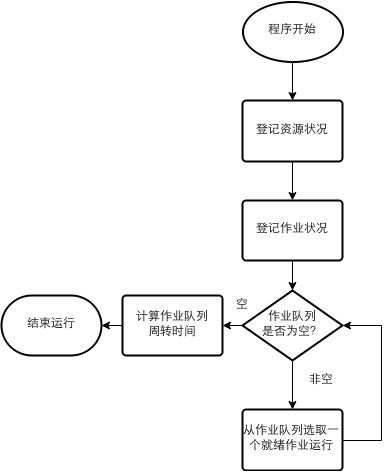
\includegraphics[scale=0.75]{figures/2.flow.png}
\end{figure}

\subsection{5、 程序调用关系}

测试程序启动之前,需要对资源进行记录。为了方便调试,实验中将所有资源状况记录到源文件中。
各个资源状态可以通过 \mintinline{c}{add_resource} 函数来进行添加。


接下来需要登记作业队列,根据实验要求,可以使用 \mintinline{c}{add_job} 来进行登记。


完成作业登记之后即可通过调用 \mintinline{c}{tick} 函数来进行作业调度。
在作业调度过程中,程序会使用 \mintinline{c}{split} 函数来将作业队列分割成:

\begin{description}
    \item{可执行调度的作业队列}
    \item{未就绪的作业队列}
    \item{已完成的作业队列}
\end{description}


接下来程序将会从可执行调度的作业队列中选取一个作业来执行(\mintinline{c}{job_run})。


完成调度之后,程序通过执行 \mintinline{c}{job_list_info}
来计算作业运行的周转时间数据情况。

\subsection{6、 数据结构及疑难描述}

\subsubsection{作业控制块}

作业控制块记录的是作业基本信息,包括以下几个字段:

\begin{table}[H]
    \centering
    \begin{tabular}{| c | c | l |}
        \hline
        字段名 & 类型 & 作用 \\ \hline
        user & char * & 用户名 \\
        name & char * & 作业名 \\
        status & int & 作业状态 \\
        atime & int & 作业就绪时间 \\
        ftime & int & 作业完成时间 \\
        rtime & int & 作业运行时间 \\
        res & struct resource * & 作业所需资源 \\ \hline
    \end{tabular}
\end{table}

\subsection{7、 程序运行结果}

根据实验要求运行指定作业:

\begin{figure}[h!]
    \centering
        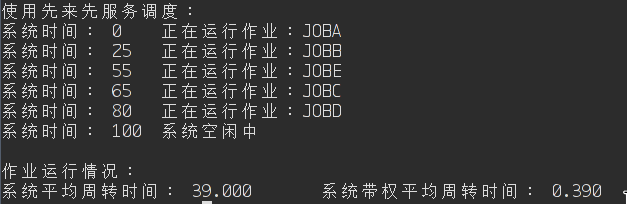
\includegraphics[scale=0.75]{figures/2.result.png}
\end{figure}

\subsection{8、 结果分析与实验小结}

通过和手工模拟的结果进行对比可以看到程序运行结果没有问题。尽管作业调度和进程调度
有很多的不同,但是从本质上来说两者没有太大区别,所以本实验可以借鉴实验一中的实现。


但另外一方面,作业调度需要考虑系统资源的分配,所以需要另外对系统资源进行跟踪,
防止因为重复分配资源导致的问题。

\clearpage

\section{实验三 可变分区分配}

\subsection{1、 实验目的}

通过编写和调试存储管理的模拟程序以加深对存储管理方案的理解。
熟悉虚存管理的各种页面淘汰算法。


通过编写和调试地址转换过程的模拟程序以加强对地址转换过程的了解。

\subsection{2、 实验内容及要求}

设计一个请求页式存储管理方案。并编写模拟程序实现之。产生一个需要访问的指令地址流。
它是一系列需要访问的指令的地址。
为不失一般性,你可以适当地(用人工指定地方法或用随机数产生器)生成这个序列,
使得 50%的指令是顺序执行的。25%的指令均匀地散布在前地址部分,
25%的地址是均匀地散布在后地址部分。


为简单起见。页面淘汰算法采用 FIFO页面淘汰算法,并且在淘汰一页时,只将该页在页表中抹去。
而不再判断它是否被改写过,也不将它写回到辅存。


\subsection{3、 实验设计方案及原理}

本实验需要将程序分为两部分,一部分用作模拟虚拟内存和物理内存的关联;
另外一部分用作生成访问地址。


\subsubsection{内存模拟}

实验中使用连续数组来表示一块内存。数组每一个项目都对应内存中的一页或一块。
这样对于虚拟页表,只需要在对应页面中保存关联的物理页面地址即可。


\subsubsection{访问地址生成}

实验中采用了先顺序、后随机的次序来生成访问地址流。内存管理程序通过读入访问地址流
即可实现对内存访问。

\clearpage

\subsection{4、 程序流程图}

\begin{figure}[h!]
    \centering
        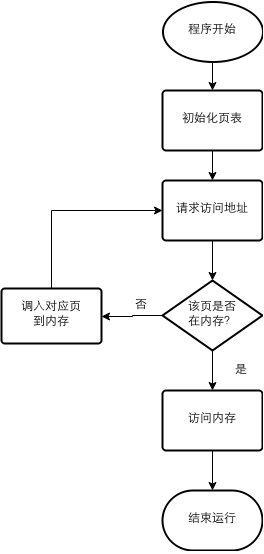
\includegraphics[scale=0.75]{figures/3.flow.png}
\end{figure}

\subsection{5、 程序调用关系}

内存模拟程序通过读入终端输入来获取访问地址。得到合法的访问地址后,会调用
\mintinline{c}{vm_hit} 函数来访问虚拟页表。


在 \mintinline{c}{vm_hit} 函数中,程序会通过调用 \mintinline{c}{PTX} 宏来计算
对应的虚拟页表,并对该页进行检索。如果该页已经调入,则直接访问对应的物理页表;
如果该页尚未调入,则会通过 \mintinline{c}{vm_alloc} 函数来进行调入操作。


程序同时采用了 MMU 实现。假如快表已满,则使用 FIFO 算法来替换一页
(使用 \mintinline{c}{phy_alloc} 函数)。


\subsection{6、 数据结构及疑难描述}

\subsubsection{内存地址结构}

\begin{description}
    \item{物理地址} 前 5 位为页面地址,后 10 位为页内偏移
    \item{虚拟地址} 前 6 位为页面地址,后 10 位为页内偏移
\end{description}

\subsubsection{页表单元}

实验中使用页表单元来记录各虚拟内存页的占用情况。该数据结构包含两个字段:

\begin{table}[H]
    \centering
    \begin{tabular}{| c | c | l |}
        \hline
        字段名 & 类型 & 作用 \\ \hline
        ppage & unsigned int & 记录物理页号 \\
        present & int & 对应页是否已加载到内存中? \\ \hline
    \end{tabular}
\end{table}

\clearpage

\subsection{7、 程序运行结果}


\begin{figure}[h!]
    \centering
        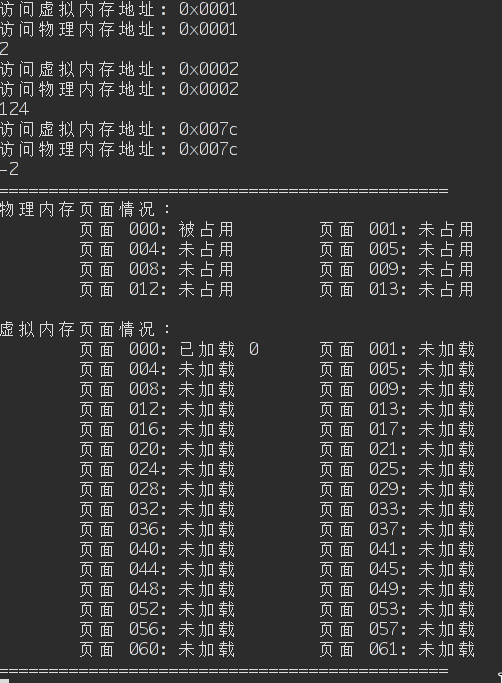
\includegraphics[scale=0.75]{figures/3.result.png}
\end{figure}

\subsection{8、 结果分析与实验小结}

通过本实验,更加深化了对虚拟内存的理解。同时根据大规模数据的测试,
我们不难发现虚拟页表的优点在于可以让程序和实际内存环境隔离,
保证了程序运行时的隔离性,让多个程序同时执行变得更加简单。

\clearpage

\section{实验四 简单文件系统}

\subsection{1、 实验目的}

用高级语言编写和调试一个简单的文件系统,模拟文件管理的工作过程。
从而对各种文件操作命令的实质内容和执行过程有比较深入的了解。


要求设计一个 n个用户的文件系统,每次用户可保存m个文件,用户在一次运行中只能打开一个文件,
对文件必须设置保护措施,且至少有 create、delete、open、close、read、write 等命令。

\subsection{2、 实验内容及要求}


设计一个10个用户的文件系统,每次用户可保存10个文件,一次运行用户可以打开5个文件。


程序采用二级文件目录(即设置主目录[MFD])和用户文件目录(UED)。
另外,为打开文件设置了运行文件目录(AFD)。

  
为了便于实现,对文件的读写作了简化,在执行读写命令时,只需改读写指针,
并不进行实际的读写操作。


\subsection{3、实验设计方案及原理}

\subsubsection{文件系统}

根据需求,实验中会在内存中开辟一块内存空间来记录系统中文件、目录情况。
其中会在执行命令的时候对文件、目录进行权限检查。

\subsubsection{用户系统}

为了实现多用户,程序需要另外记录系统中的用户列表。并在操作文件、目录的时候
对目标文件、目录写入相关权限信息。


通过上述两个部分的实现,程序即可以模拟操作系统中的系统调用来操纵文件系统。

\clearpage

\subsection{4、 程序流程图}

\begin{figure}[h!]
    \centering
        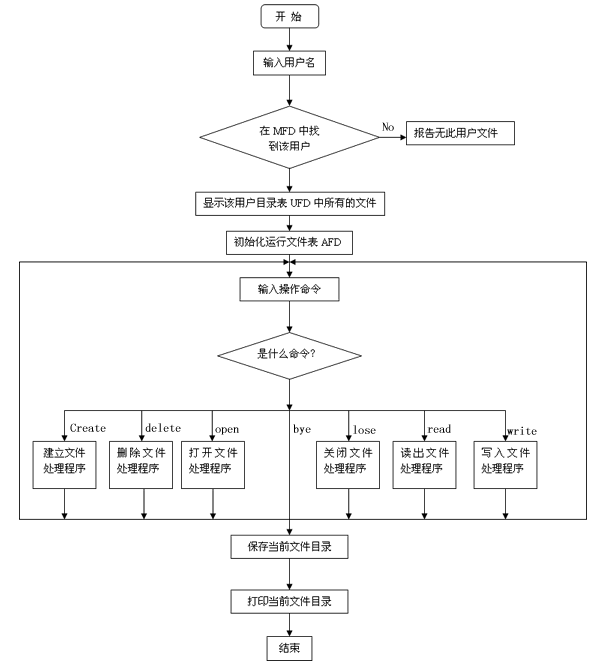
\includegraphics[scale=0.75]{figures/4.flow.png}
\end{figure}


\subsection{5、 程序调用关系}

程序启动前,需要调用 \mintinline{c}{user_get_by_id}、 \mintinline{c}{useradd} 
等函数来初始化用户系统。


接着需要通过调用 \mintinline{c}{create} 等文件系统操作指令来初始化基本目录。


最后启动一个简单的 shell 程序(通过 \mintinline{c}{repl} 函数)来读入用户指令,
并根据用户意图来执行对应文件系统操作指令来实现用户交互操作。

\subsection{6、 数据结构及疑难描述}

\subsubsection{文件记录块}

为了记录文件系统中的文件情况,需要通过文件记录块来保存相关信息。
该数据结构包含以下字段:

\begin{table}[H]
    \centering
    \begin{tabular}{| c | c | l |}
        \hline
        字段名 & 类型 & 作用 \\ \hline
        name & char * & 记录名称 \\
        type & int & 记录类型(文件、目录、未分配) \\
        owner\_id & int & 记录所有者的 id \\
        owner\_perm & int & 记录所有者的访问权限 \\
        other\_perm & int & 非记录所有者的访问权限 \\
        parent & 记录指针 & 该记录的父记录结点 \\
        files & 子记录指针 & 该记录下的子记录(仅为目录类型时有效)\\
        count & int & 子记录数量 (仅为目录类型时有效) \\
        content & char * & 记录内容(仅为文件类型时有效) \\ \hline
    \end{tabular}
\end{table}

\clearpage

\subsection{7、 程序运行结果}

\begin{figure}[h!]
    \centering
        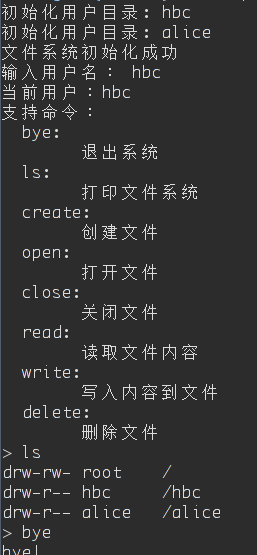
\includegraphics[scale=0.75]{figures/4.result.png}
\end{figure}

\subsection{8、 结果分析与实验小结}

通过一系列的模拟操作,可以看到该模拟文件系统可以按照预期正常工作。在这个实验中,
模拟文件系统的实现加深了我对操作系统对资源的管理实现机制的理解。
而且可以感受到各个文件系统采取不同设计的原因。


通过实验的编程,也提高了我的编码能力。

\end{document}
